\chapter{PCB Design}
\label{chap7}
Printed Circuit Board (PCB) \index{PCB} design is a very important step in electronic system design. Every component of your circuit needs to be placed and connections routed to minimize delay and area. Each component has an associated footprint. Footprint refers to the physical layout of a component that is required to mount it on the PCB.\index{Component!footprint} \index{Footprints} PCB design involves mapping footprints for all components, placing them appropriately to minimize wire length and area, connecting the footprints using tracks/vias and finally extracting the required files needed for printing the PCB. Let us see the steps to design PCB using Oscad.
\section{Schematic Creation for PCB design}
In chapter \ref{chap5}, we have seen the differences between schematic for simulation and schematic for PCB design. Let us take the example of an RC low pass circuit. We have used a resisitor, capacitor, a sinusoidal voltage source, ground, plots, and power flag. Note that the sinusoidal voltage source and plot components were fictitious components added to let the simulator know what kind of simulation to do and what kinds of signals need to be plotted. These components are not needed for PCB design. You would need to connect an external signal generator instead of the fictitious sinusoidal source. You also do not need a plot component in a PCB. So let us modify the schematic of RC circuit created in chapter \ref{chap5} for PCB design. Before doig this, you may want to make a back up copy of the files created in Chapter \ref{chap5} to prevent them getting overwritten.

Open the RC circuit schematic in Schematic editor. Delete the sinusoidal voltage source and plot blocks and place a two pin connector, \textit{CONN\_2} from the EEschema library \textit{conn}. You can use the delete key to delete components or you can right-click on the component and choose \textit{Delete compoenent}. See section \ref{sconn} to know more about EEschema library \textit{conn}. Connect the components, and make the final schematic as shown in Figure \ref{pcbschfin}. Do the annotation and test for ERC. Please refer to chapter \ref{chap5} to know more about basic steps in schematic creation.
\begin{figure}
\centering
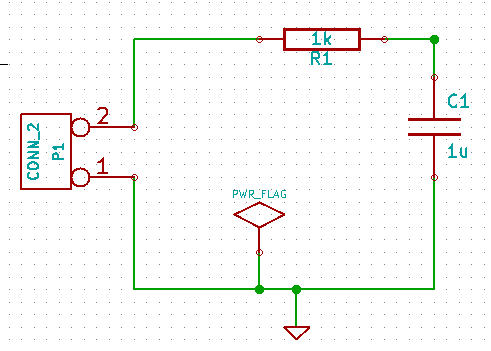
\includegraphics[width=0.7\textwidth]{figures/pcbschfin}
\caption{Final circuit schematic for RC low pass circuit}
\label{pcbschfin}
\end{figure}
\subsection{Netlist generation for PCB}
\index{Netlist!for PCB}
\label{netc}
The netlist for PCB is different from that for simulation. To generate netlist for PCB, click on the \textit{Generate netlist} tool from the top toolbar in Schematic editor. Click on the button \textit{Netlist} under the tab \textit{Pcbbew} in the Netlist window. This is shown in Figure \ref{netlistpcb}. Click on \textit{Save} in the Save netlist file dialog box that opens up. Do not change the directory or the name of the netlist file. 

\begin{figure}
\centering
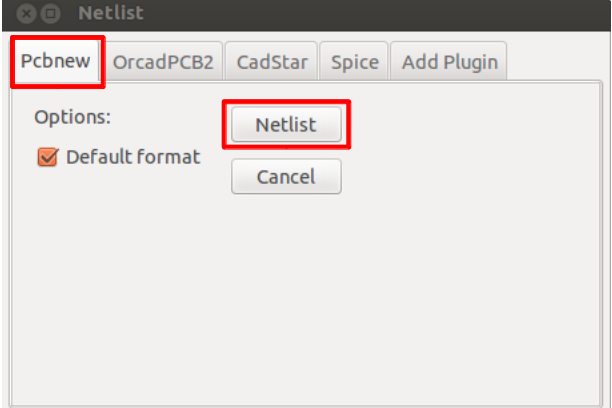
\includegraphics[width=0.7\textwidth]{figures/netlistpcb}
\caption{Netlist generation for PCB}
\label{netlistpcb}
\end{figure}
\textit{Note that the netlist has an extension `.net'. The netlist created for simulation had an extension `.cir'}.

Save the schematic and close the schematic editor.
\subsection{Mapping of Components using Footprint Editor}
\index{Footprints!mapping}
\index{Component!footprint!mapping}
Once the netlist for PCB is created, you need to map each component in the netlist with a footprint. The tool {\tt Footprint Editor} is used for this. Oscad uses {\tt CvPcb} as its footprint editor. CvPcb is the footprint editor tool in KiCad.
\subsection{Familiarising the Footprint Editor tool}
\index{Footprint editor}
If you open the Footprint editor after creating the {\tt .net} netlist file, you will get the Footprint editor as shown in Figure \ref{fe}. The menu and tool bars and the panes are marked in this figure. The menu bar will be available in the top left corner. The left pane has a list of components in the netlist file and the right pane has a list of available footprints for each component.

\begin{figure}
\centering
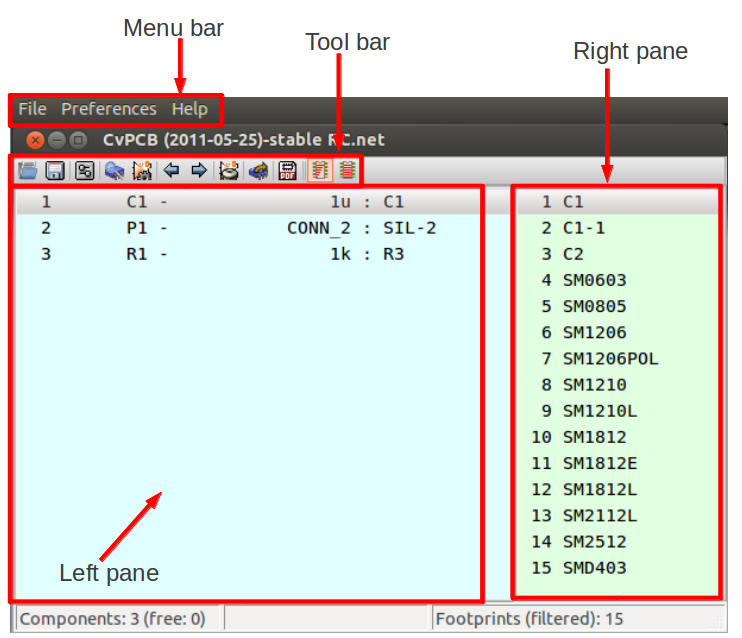
\includegraphics[width=0.7\textwidth]{figures/fe}
\caption{Footprint editor with the menu and tool bars and the left and right panes marked}
\label{fe}
\end{figure}
\textit{Note that if you open the Footprint editor before creating a `.net' file, then the left and right panes will be empty}.
\subsubsection{Tool bar}
Some of the important tools in the tool bar are shown in Figure \ref{tb_fe}. They are explained below:
\begin{figure}
\centering
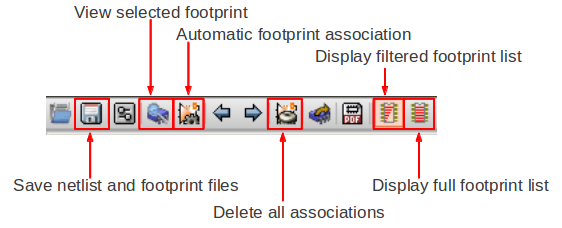
\includegraphics[width=0.7\textwidth]{figures/tb_fe}
\caption{Some important tools in the tool bar}
\label{tb_fe}
\end{figure}
\begin{enumerate}
\item Save netlist and footprint files - Save the netlist and the footprints that you have associated with it.
\item View selected footprint - View the selected footprint in 2D. See section \ref{viewfp} for more details.
\item Automatic footprint association - Perform footprint association to each component automatically. Footprints will be selected from the list of footprints available.
\item Delete all associations - Delete all the footprint associations made
\item Display filtered footprint list - Display a filtered list of footprints suitable to the selected component
\item Display full footprint list - Display the list of all footprints available (without filtering)
\end{enumerate}
\subsection{Viewing footprints in 2D and 3D}
\index{Footprints!view!2D}
\index{Footprints!view!3D}
\label{viewfp}
To view a footprint in 2D, choose the footprint from the right pane and click on \textit{View selected footprint} from the menu bar. Let us view the footprint for {\tt SM1210}. Choose SM1210 from the right pane as shown in Figure \ref{sm}. On clicking the View selected footprint tool, you will get the Footprint window with the view in 2D. Click on the \textit{3D} tool in the footprint window, as shown in Figure \ref{3d}. You will now get a top view of the selected footprint in 3D. Click on the footprint and rotate it using mouse to get 3D views from various angles. One such side view of the footprint in 3D is shown in Figure \ref{3dv}.
\begin{figure}
\centering
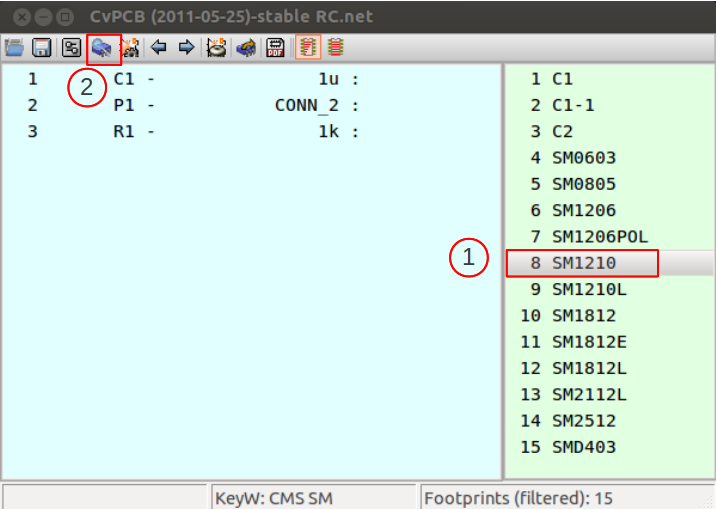
\includegraphics[width=0.7\textwidth]{figures/sm}
\caption{1. Choose the footprint SM1210 from the right pane, then 2. click on View selected footprint}
\label{sm}
\end{figure}
\begin{figure}
\centering
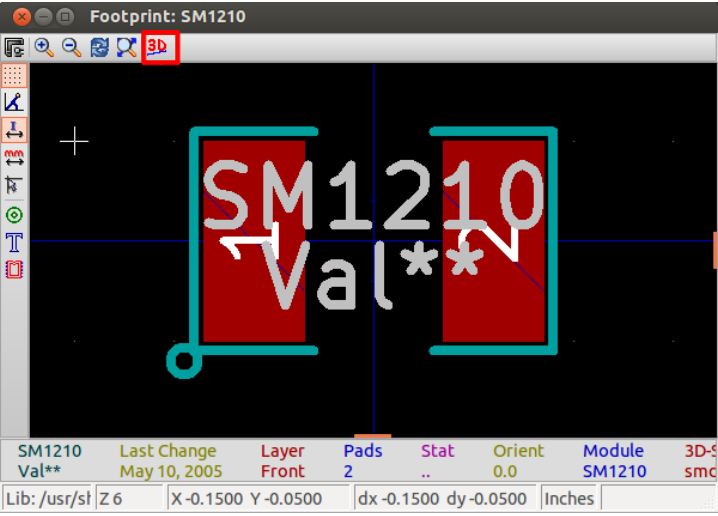
\includegraphics[width=0.7\textwidth]{figures/3d}
\caption{Footprint view in 2D. click on 3D to get 3D view}
\label{3d}
\end{figure}
\begin{figure}
\centering
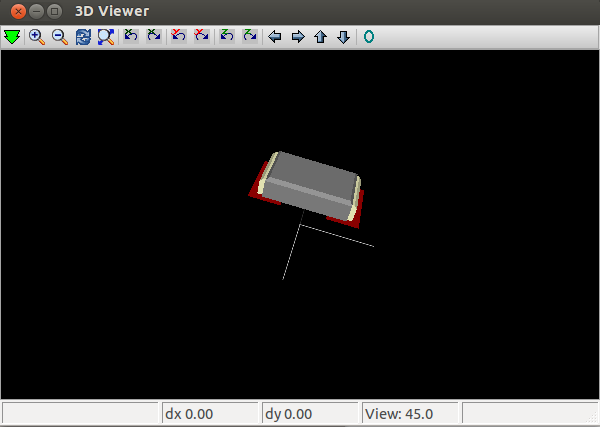
\includegraphics[width=0.7\textwidth]{figures/3dv}
\caption{Rotate the footprint upwards to get the 3D view from a different angle}
\label{3dv}
\end{figure}
\subsection{Mapping of components in the RC circuit}
Click on {\tt C1} from the left pane. Choose the footprint \textit{C1} from the right pane by double-clicking on it. Click on connector {\tt P1} from the left pane. Choose the footprint \textit{SIL-2} from the right pane by double-clicking on it. Similarly choose the footprint \textit{R3} for the resistor {\tt R1}. The footprint mapping is shown in Figure \ref{map}. Save the footprint association by clicking on the \textit{Save netlist and footprint files} tool form the toolbar. The {\tt Save Net and component List} window appears. Browse to the directory where you have saved your schematic file for this project and click on {\tt Save}. The netlist gets saved and the Footprint editor window closes automatically.

\begin{figure}
\centering
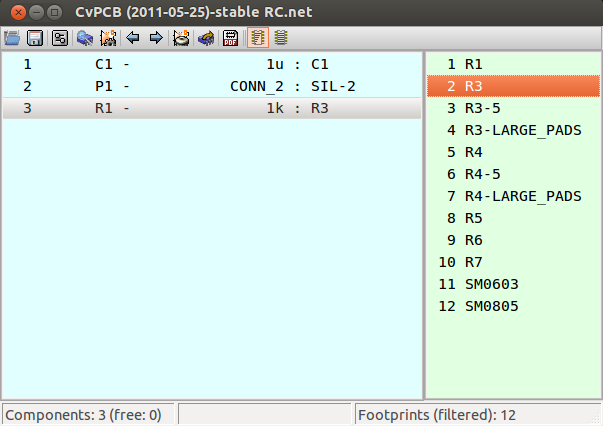
\includegraphics[width=0.7\textwidth]{figures/map}
\caption{Footprint mapping done}
\label{map}
\end{figure}
\textit{Note that you need to browse to the directory where you saved the schematic file to save the `.net' file}.
\section{Creation of PCB Layout}
\index{PCB Layout!creation}
The next step is to place the footprints and lay tracks between them to get the layout. This is done using the {\tt Layout Editor} tool. Oscad uses {\tt Pcbnew}, the layout creation tool in KiCad, as its layout editor.
\subsection{Familiarising the Layout Editor Tool}
\index{Layout editor}
The Layout editor with the various menu and tool bars is shown in Figure \ref{pcbnew}.
\begin{figure}
\centering
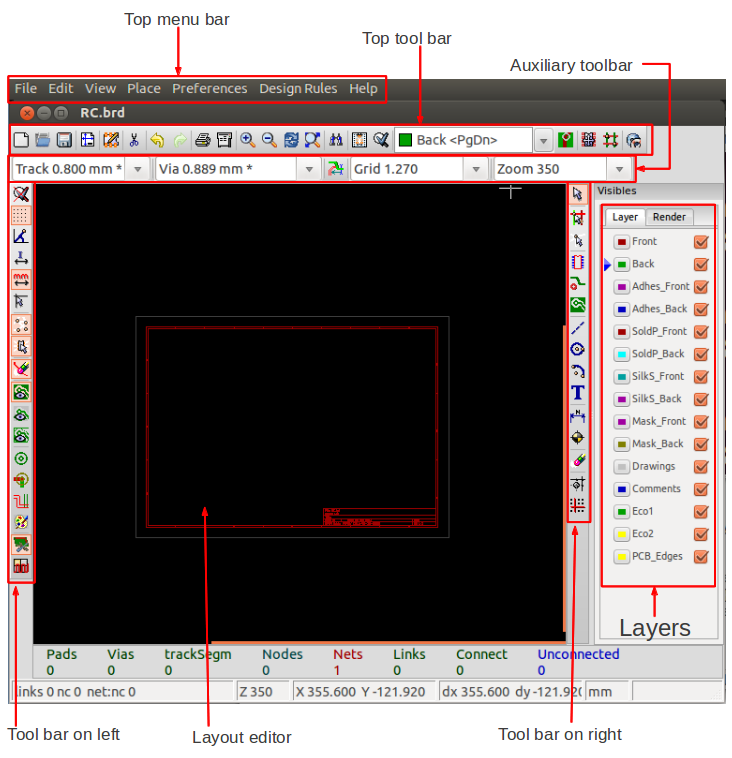
\includegraphics[width=0.7\textwidth]{figures/pcbnew}
\caption{Layout editor with menu and tool bars and the layer options marked}
\label{pcbnew}
\end{figure}
\begin{figure}
\centering
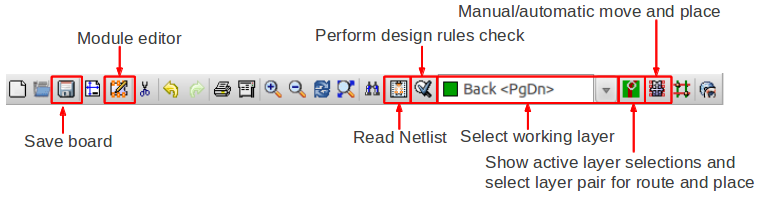
\includegraphics[width=0.9\textwidth]{figures/toptble}
\caption{Top toolbar with important tools marked}
\label{toptble}
\end{figure}
\subsubsection{Top tool bar}
Some of the important menu options in the top menu bar are shown in Figure \ref{toptble}. They are explained below:
\begin{enumerate}
\item Save board - Save the printed circuit board
\item Module editor - Open module editor to edit footprint modules or libraries
\item Read Netlist - Import the netlist whose layout needs to be created.
\item Perform design rules check - Check for design rules, unconnected nets etc. in the layout made.
\item Select working layer - Selection of working layer
\item Show active layer selections and select layer pair for route and place - Select layer in top and bottom layers. It also shows currently active layer selections.
\item Mode footprint: Manual/automatic move and place - Move and place modules
\end{enumerate}
\subsection{Hotkeys}
\index{Hotkeys!Layout editor}
A list of hotkeys are given below:
\begin{enumerate}
\item F1 - Zoom in
\item F2 - Zoom out
\item Delete - Delete Track or Footprint
\item  X - Add new track
\item V - Add Via
\item M - Move Item
\item F - Flip Footprint
\item R - Rotate Item
\item G - Drag Footprint
\item Ctrl+Z - Undo
\item E - Edit Item
\end{enumerate}
The list can be viewd by selecting \textit{Preferences} from the top menu bar and choosing \textit{List Current Keys} from the option \textit{Hotkeys}.
\subsection{PCB design example using RC circuit}
Click on Layout Editor from the Oscad toolbar. Click on \textit{Read Netlist} tool from the top tool bar. Click on \textit{Browse Netlist files} on the Netlist window that opens up. Select the {\tt RC.net} file that we have saved after assigning footprints. Click on \textit{Open}. Now Click on \textit{Read Current Netlist} on the Netlist window. The message area in the Netlist window says that the RC.net has been read. The sequence of operations is shown in Figure \ref{brnet}.

\begin{figure}
\centering
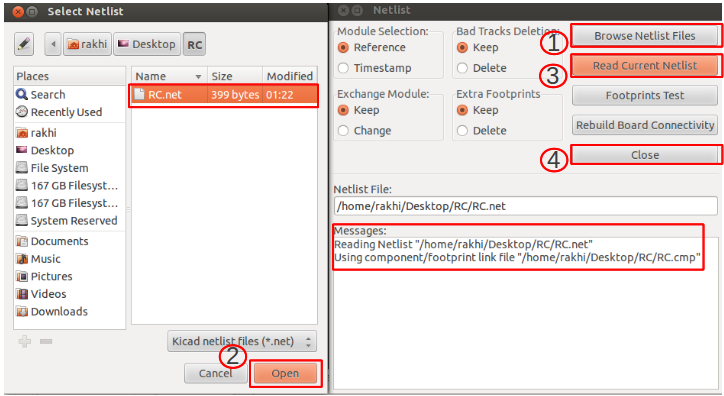
\includegraphics[width=0.7\textwidth]{figures/brnet}
\caption{Importing netlist file to layout editor. 1. Browse netlist Files 2. Choose the RC.net file 3. Read Netlist file 4. Close}
\label{brnet}
\end{figure}

The footprint modules will now be imported to the top left hand corner of the Layout Editor. This is shown in Figure \ref{netlisttop}.
\begin{figure}
\centering
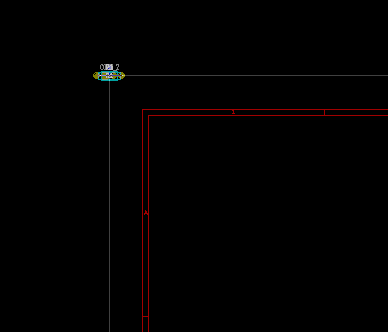
\includegraphics[width=0.7\textwidth]{figures/netlisttop}
\caption{Footprint modules imported to top left corner of Layout Editor}
\label{netlisttop}
\end{figure}
Zoom in  to the top left corner by pressing the key {\tt F1} or using the scroll button of your mouse. The Zoomed in version of the imoprted netlist is shown in Figure \ref{zoom}. Let us now place this in the center of the Layout editor window.
\begin{figure}
\centering
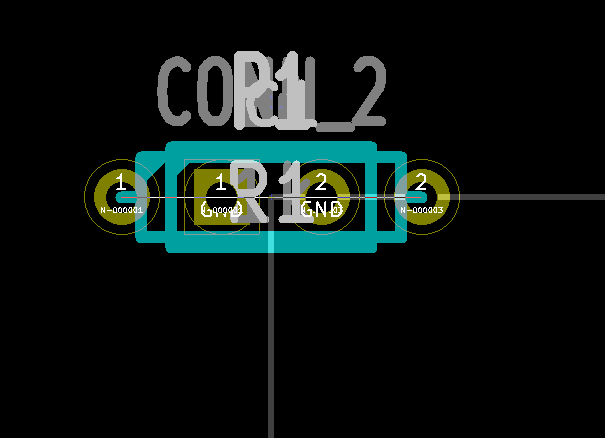
\includegraphics[width=0.7\textwidth]{figures/zoom}
\caption{Zoomed in version of the imported netlist}
\label{zoom}
\end{figure}
Click on \textit{Mode footprint: Manual/automatic move and place} tool from the top tool bar. Place the cursor near the center of the layout editor window.
Right click and choose \textit{Glob move and place}. Choose \textit{move all modules}. The sequence of operations is shown in Figure \ref{movep}. Click on yes on the confirmation window, as shown in Figure \ref{confirm}, to move the modules.
 Zoom in using the F1 key. The current placement of components after zooming in is shown in Figure \ref{curplace}.
\begin{figure}
\centering
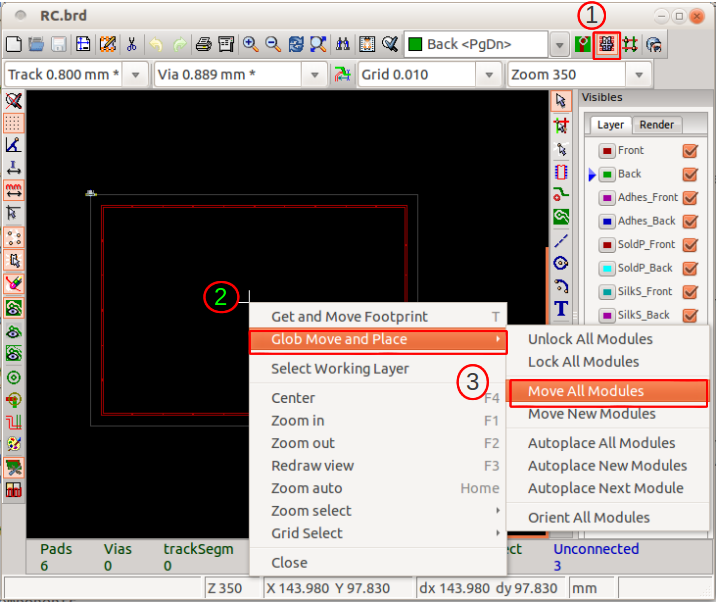
\includegraphics[width=0.7\textwidth]{figures/movep}
\caption{Move and place modules to center of layout editor. 1. Click on Mode footprint: Manual/automatic move and place 2. Place cursor at center of layout editor and right click on it 3. Choose Glob move and place and then choose move all modules.}
\label{movep}
\end{figure}
\begin{figure}
\centering
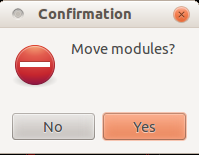
\includegraphics[width=0.3\textwidth]{figures/confirm}
\caption{Click on Yes in the confirmation window}
\label{confirm}
\end{figure}
\begin{figure}
\centering
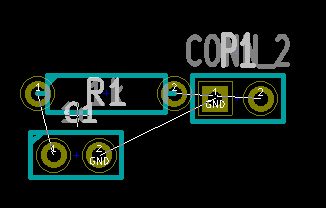
\includegraphics[width=0.4\textwidth]{figures/curplace}
\caption{Zoomed in version of the current placement after moving modules to the center of the layout editor}
\label{curplace}
\end{figure}

We need to arrange the modules properly to lay tracks. Rotate the connector P1 by placing the cursor on top of P1 and pressing R. Move it by placing the cursor on top of it and pressing M. The final placement is shown in Figure \ref{fplace}.
\index{Footprints!move and place}
\begin{figure}
\centering
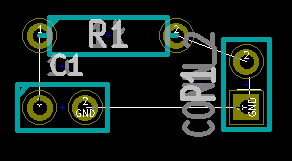
\includegraphics[width=0.4\textwidth]{figures/fplace}
\caption{Final placement of footprints after rotating and moving P1}
\label{fplace}
\end{figure}

Let us now lay the tracks. Let us first change the track width. Click on \textit{Design rules} from the top menu bar. Click on design rules. This is shown in Figure \ref{drules}. The \textit{Design Rules Editor} window opens up. Here you can edit the various design rules. Double-click on the track width field to edit it. Type 0.8 and press Enter. Click on ok. Figure \ref{druleedit} shows the sequence of operations. 
\index{PCB design!lay tracks}
\index{PCB design!design rules}
\begin{figure}
\centering
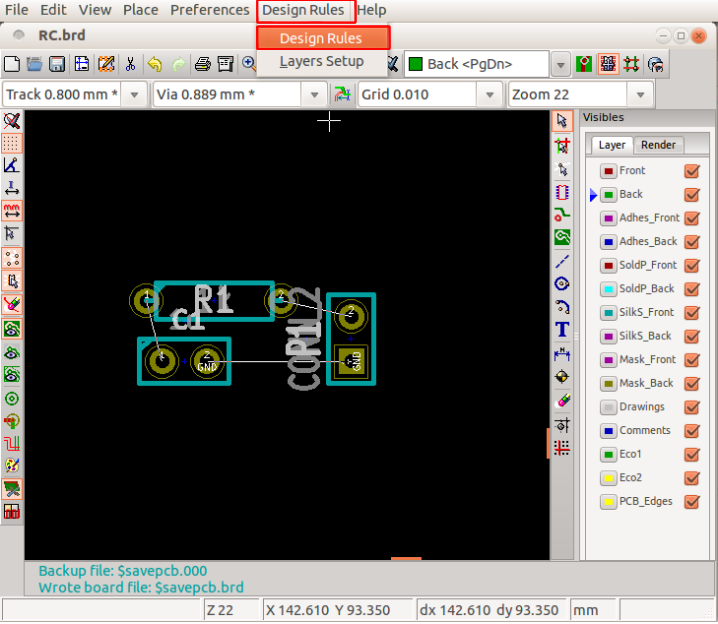
\includegraphics[width=0.7\textwidth]{figures/drules}
\caption{Choose Design rules from the top menu bar and choose design rules}
\label{drules}
\end{figure}
\begin{figure}
\centering
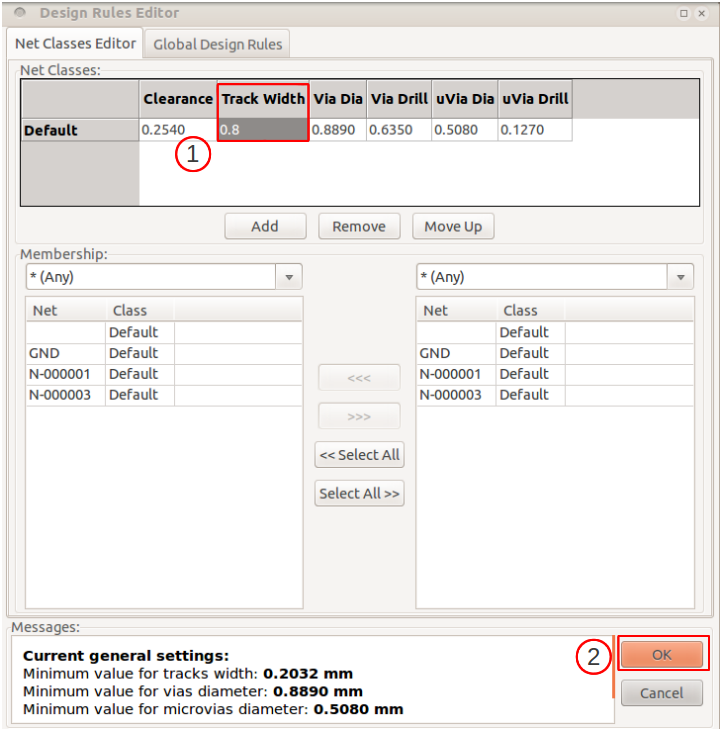
\includegraphics[width=0.7\textwidth]{figures/druleedit}
\caption{1. Double-click on track width field and type 0.8, 2. Click on ok}
\label{druleedit}
\end{figure}

Click on \textit{Back} from the \textit{Layer} options as shown in Figure \ref{layer}.
\begin{figure}
\centering
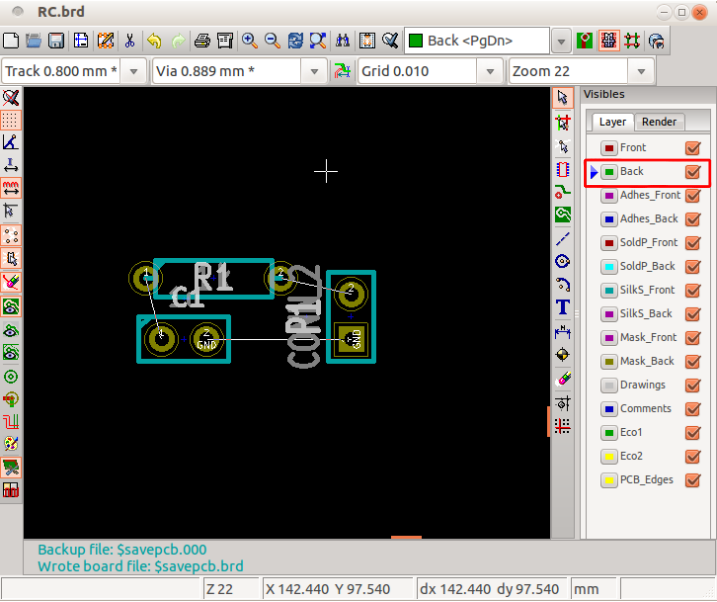
\includegraphics[width=0.6\textwidth]{figures/layer}
\caption{Choose the copper layer `Back'}
\label{layer}
\end{figure}

Let us now start laying the tracks. Place the cursor above the left terminal of R1 in the layout editor. Press the key {\tt x}.
Move the cursor down and double-click on the left terminal of C1. A track is formed. This is shown in \figref{track1}.
\begin{figure}
\centering
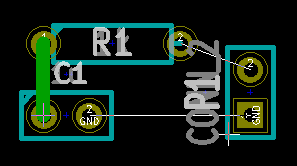
\includegraphics[width=0.4\textwidth]{figures/track1}
\caption{A track formed between resistor and capacitor}
\label{track1}
\end{figure}

Similarly lay the track between capacior C1 and connector P1 as shown in \figref{track2}.
\begin{figure}
\centering
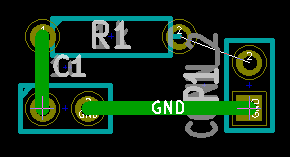
\includegraphics[width=0.4\textwidth]{figures/track2}
\caption{A track formed between capacitor and connector}
\label{track2}
\end{figure}
The last track needs to be laid at an angle. To do so, place the cursor above the second terminal of R1. Press the key x and move the cursor diagonally down. Double-click on the other terminal of connector. The track will be laid as shown in \figref{track3}.
\begin{figure}
\centering
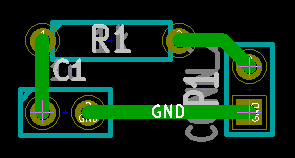
\includegraphics[width=0.4\textwidth]{figures/track3}
\caption{A track formed between connector and resistor}
\label{track3}
\end{figure}
All tracks are now laid. The next step is create PCB edges. 

Choose \textit{PCB\_edges} from the Layer options to add edges. Choose \textit{Add graphic line or polygon} from the toolbar on the left. \figref{pcbedges} shows the sequence of operations. Let us now start drawing edges for PCB.
\index{PCB design!pcb edges}
\begin{figure}
\centering
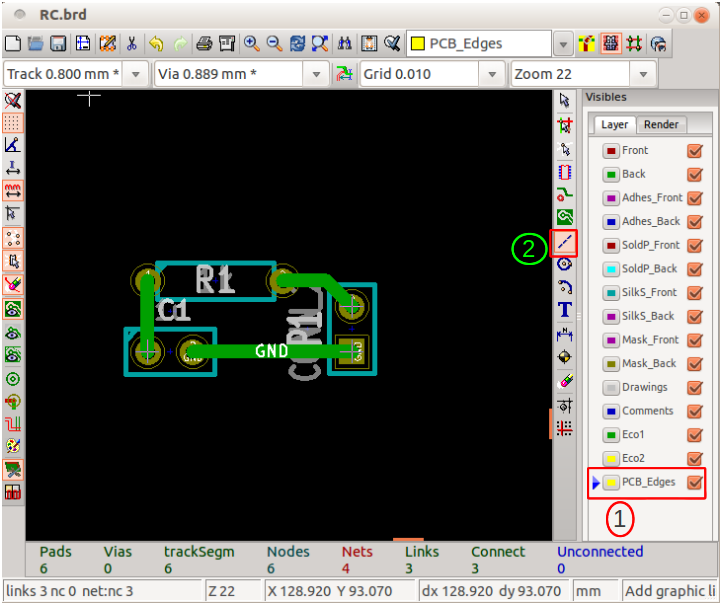
\includegraphics[width=0.7\textwidth]{figures/pcbedges}
\caption{1. Choose PCB\_edges from Layer options 2. Choose Add graphic line or polygon from left toolbar}
\label{pcbedges}
\end{figure}
Click to the left of the layout. Move cursor horizontally to the right. Click once to change orientation. Move cursor vertically down. Draw  the edges as shown in Figure \ref{pcbed}. Double-click to finish drawing edges.
\begin{figure}
\centering
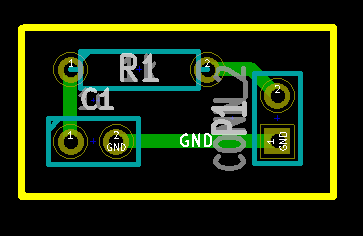
\includegraphics[width=0.4\textwidth]{figures/pcbed}
\caption{PCB edges drawn}
\label{pcbed}
\end{figure}

Click on \textit{Perform design rules check} from the top tool bar to check for design rules. The \textit{DRC Control} window opens up. Click on \textit{Start DRC}. There are no errors under the Error messages tab. Click on ok to close DRC control window. The figure \ref{drc} shows the sequence of operations.
\index{PCB design!design rules check}
\begin{figure}
\centering
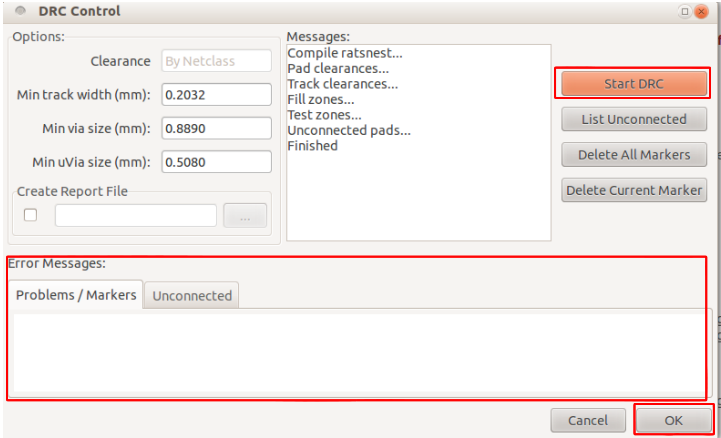
\includegraphics[width=0.7\textwidth]{figures/drc}
\caption{1. Click on Start DRC 2. Click on Ok}
\label{drc}
\end{figure}

Click on \textit{Save board} on the top toolbar. To generate gerber files, click on \textit{File} from the top menu bar. Click on \textit{plot}. This is shown in Figure \ref{plot}. The plot window opens up. You can choose which layers to plot by selecting/deselecting them from the left side.
You can also choose the format to plot. Choose Gerber. The output directory of the plots created can also be chosen. By default, it is the project directory. Some more options can be chosen in this window. Click on \textit{Plot}. The message window shows the location in which Gerber files are created. Click on Close. This is shown in Figure \ref{plot2}.\index{PCB design!gerber}
\begin{figure}
\centering
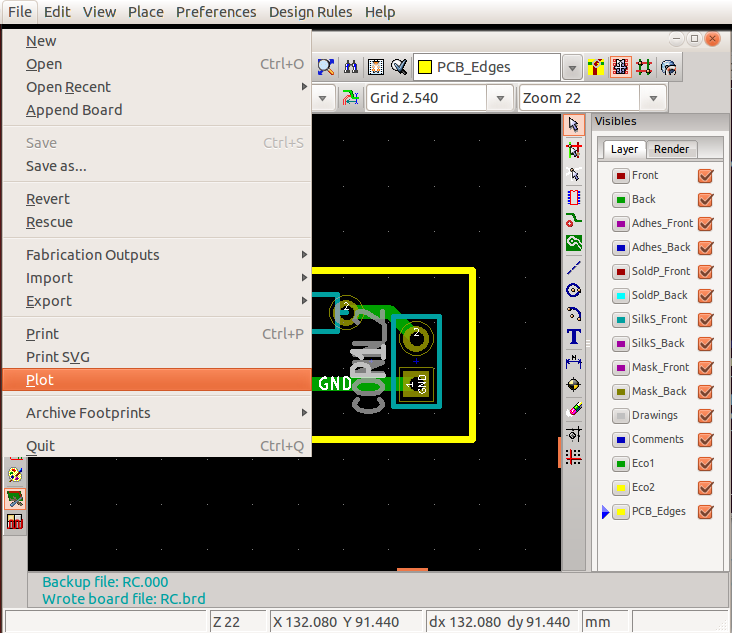
\includegraphics[width=0.7\textwidth]{figures/plot}
\caption{Choose plot from the File menu}
\label{plot}
\end{figure}
\begin{figure}
\centering
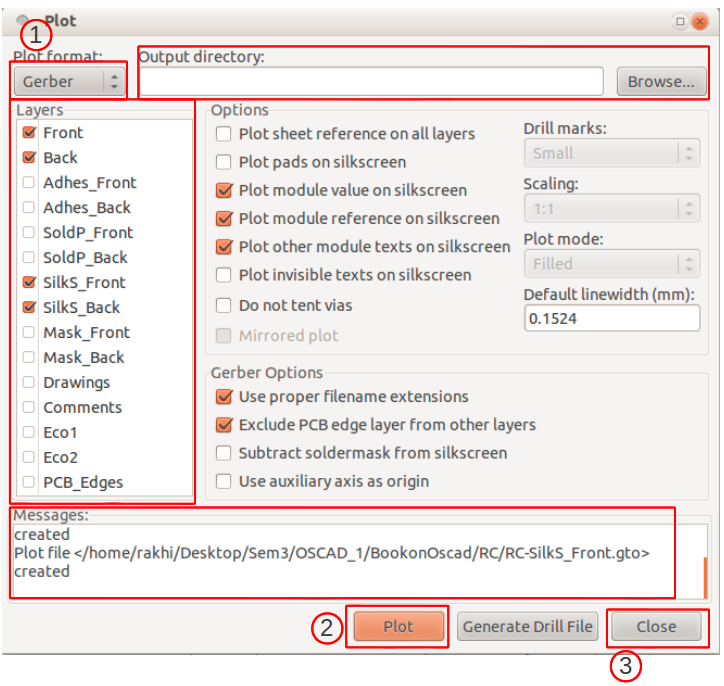
\includegraphics[width=0.7\textwidth]{figures/plot2}
\caption{1. Choose Gerber as the plot format 2. Click on Plot. Message window shows location in which Gerber files are created 3. Click on Close}
\label{plot2}
\end{figure}

The PCB design of RC circuit is now complete. If you would like to know more about Pcbnew, please refer \cite{eeschema}.

